\documentclass[11pt,a4paper]{article}

% ============================================================
% JSD TATA Emergency Services
% Power BI Analytics & Data Engineering
% Compile: pdflatex PowerBI-DataEngineering.tex  (run twice for TOC)
% ============================================================

\usepackage[margin=1in]{geometry}
\usepackage{xcolor}
\usepackage{titlesec}
\usepackage{tabularx}
\usepackage{booktabs}
\usepackage{array}
\usepackage{enumitem}
\usepackage{listings}
\usepackage{fancyhdr}
\usepackage{tikz}
\usetikzlibrary{shapes.geometric, arrows.meta, positioning}
\usepackage{hyperref}

% ---- brand palette ----
\definecolor{accent}{HTML}{07514D}
\definecolor{accent2}{HTML}{2E8B84}
\definecolor{ink}{HTML}{0F172A}
\definecolor{muted}{HTML}{64748B}
\definecolor{soft}{HTML}{EEF2F1}
\definecolor{blue}{HTML}{2563EB}
\definecolor{pink}{HTML}{BE185D}
\definecolor{line}{HTML}{CBD5E1}

\hypersetup{colorlinks=true, linkcolor=accent, urlcolor=blue, pdftitle={Power BI Analytics and Data Engineering}}

% ---- section styling ----
\titleformat{\section}{\color{ink}\Large\bfseries}{\color{accent}\thesection}{0.6em}{}
\titleformat{\subsection}{\color{accent}\large\bfseries}{\thesubsection}{0.6em}{}
\titlespacing*{\section}{0pt}{1.4em}{0.6em}

% ---- header / footer ----
\pagestyle{fancy}
\fancyhf{}
\renewcommand{\headrulewidth}{0pt}
\renewcommand{\footrulewidth}{0.4pt}
\fancyfoot[L]{\footnotesize\color{muted} JSD TATA Emergency Services \,\textperiodcentered\, Power BI \& Data Engineering}
\fancyfoot[R]{\footnotesize\color{muted} Page \thepage}

% ---- listings (code) ----
\lstdefinestyle{code}{
  basicstyle=\ttfamily\footnotesize\color{white},
  backgroundcolor=\color{ink},
  frame=none, breaklines=true, columns=fullflexible,
  xleftmargin=8pt, xrightmargin=8pt, framexleftmargin=8pt,
  aboveskip=8pt, belowskip=8pt, showstringspaces=false,
}
\lstset{style=code}

% ---- note box ----
\newcommand{\notebox}[1]{%
  \par\vspace{4pt}\noindent
  \colorbox{soft}{\begin{minipage}{\dimexpr\linewidth-2\fboxsep}%
  \color{ink}\small\textbf{Note.} #1\end{minipage}}\par\vspace{6pt}}

\newcolumntype{L}[1]{>{\raggedright\arraybackslash}p{#1}}

\renewcommand{\arraystretch}{1.3}

\begin{document}

% ============================================================
% TITLE PAGE
% ============================================================
\begin{titlepage}
\noindent
\colorbox{accent}{\begin{minipage}[t][3.2cm][c]{\dimexpr\textwidth-2\fboxsep}
  \color{white}\hspace{4pt}
  {\footnotesize\textbf{\textsf{JSD TATA EMERGENCY SERVICES}}}\\[10pt]
  \hspace{4pt}{\Huge\bfseries Power BI Analytics \&\\ \hspace{4pt}Data Engineering}
\end{minipage}}

\vspace{6pt}
\noindent{\large\color{muted} Turning live emergency-response data into business insight}

\vspace{2cm}
\noindent\color{ink}\small
A combined business and engineering document: what the platform measures and the
decisions it enables, followed by the end-to-end data-engineering workflow that powers
the Power BI reports --- sources, Web-connector ingestion, Power Query transformations,
the data model, DAX, refresh, and the analytics design (including advanced Power BI
capabilities).

\vfill
\noindent\textcolor{line}{\rule{\textwidth}{0.5pt}}\\[6pt]
\begin{tabular}{@{}ll@{}}
\textbf{Document} & Power BI Analytics \& Data Engineering \\
\textbf{Date} & 29 June 2026 \\
\textbf{Audience} & Business leadership (with engineering detail) \\
\textbf{Status} & Confidential --- internal \\
\end{tabular}
\end{titlepage}

% ============================================================
% CONTENTS
% ============================================================
\tableofcontents
\newpage

% ============================================================
% 1. EXECUTIVE SUMMARY
% ============================================================
\section{Executive summary}
JSD TATA Emergency Services coordinates ambulances, fire trucks and blood-bank logistics
across the Jamshedpur township. Every booking, dispatch, ETA and completion is captured as
live operational data. This document describes how that data is engineered into Power BI and
the business insights it surfaces --- response performance, fleet readiness, demand patterns,
fuel economics and service-level compliance --- so leadership can act on facts, not guesswork.

Analytics is delivered two ways: an embedded dashboard inside the operations app (no separate
Power BI login, authorised by the same corporate SSO), and the full Power BI report for deeper
analysis. The data is sourced directly from the platform's live API using Power BI Web
connectors, so reports reflect real operations with no manual exports.

% ============================================================
% 2. WHAT WE MEASURE
% ============================================================
\section{What we measure \& why it matters}
\begin{tabularx}{\textwidth}{L{0.34\textwidth} X}
\toprule
\rowcolor{soft}\textbf{Metric} & \textbf{What it tells the business} \\
\midrule
Total responses \& today's volume & Service demand and load trend over time. \\
Active vs queued incidents & Whether current capacity meets live demand. \\
Avg response time (to scene) & How fast help arrives --- the core service promise. \\
SLA compliance \% & Share of incidents met within target by severity (Critical 8 / Urgent 15 / Normal 30 min). \\
Responses by severity \& type & Case mix --- medical vs fire, Critical/Urgent/Normal. \\
Responses by zone & Geographic demand hotspots for resource placement. \\
Fleet utilisation & How hard the fleet is working; spare capacity. \\
Fuel burn \& refuel cadence & Operating-cost driver and readiness risk (low-fuel units). \\
Band-based entitlements & Transport allotment governance by employee band (0--4). \\
\bottomrule
\end{tabularx}

% ============================================================
% 3. SERVICES & DATA
% ============================================================
\section{Services \& data the platform produces}
All analytics draw from one platform. The table maps each service to the data it contributes
to the reporting layer.

\begin{tabularx}{\textwidth}{L{0.36\textwidth} X}
\toprule
\rowcolor{soft}\textbf{Service / source} & \textbf{Data contributed to analytics} \\
\midrule
Dispatch API (psiog-transport-api) & Emergencies, requests, bookings, status, severity, ETA, distance, assignments. \\
Fleet (DynamoDB) & Vehicles, drivers, status, fuel level, tank/consumption, refuel flags. \\
ReferenceData (DynamoDB) & Zones, hospitals, fire stations, locations, dispatch policy. \\
jamshedpur-users (shared) & Employee directory and band (0--4) for entitlement analytics. \\
Hospital integration & Inbound hospital ambulance requests (source = HOSPITAL). \\
Fuel-team integration & Refuel confirmations and litres dispensed (fuel logs). \\
Voice agent (Bedrock) & Voice-originated bookings (source-channel mix). \\
\bottomrule
\end{tabularx}

% ============================================================
% PIPELINE DIAGRAM
% ============================================================
\section{Power BI data pipeline}
How operational data flows from the live API into business-ready visuals.

\vspace{6pt}
\begin{center}
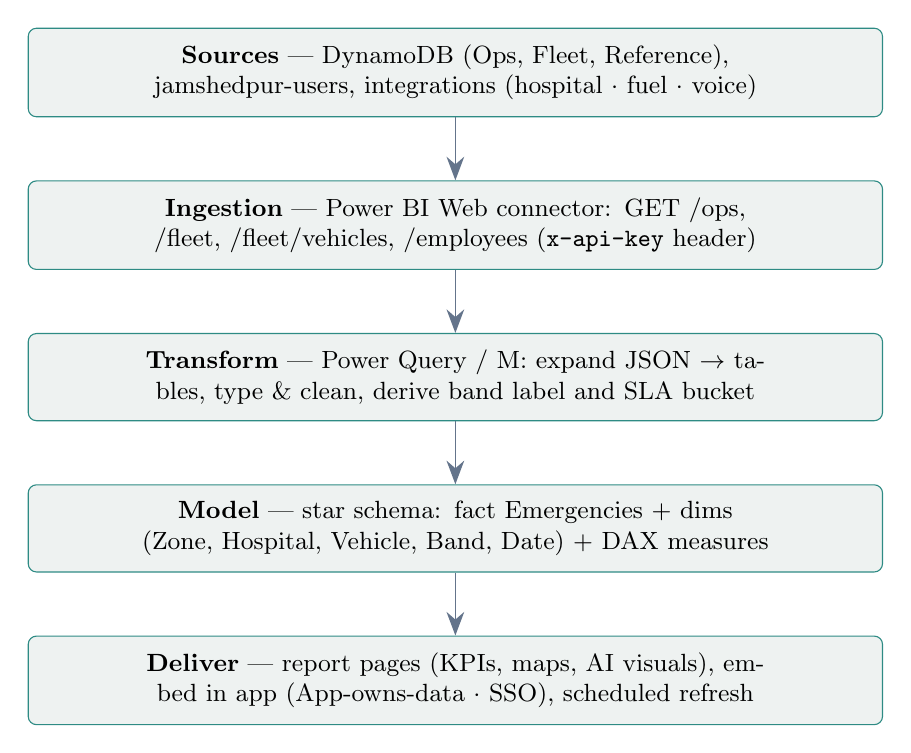
\begin{tikzpicture}[
  node distance=8mm,
  stage/.style={rectangle, rounded corners=3pt, draw=accent2, fill=soft,
    text width=0.86\textwidth, align=center, inner sep=6pt, font=\small},
  lbl/.style={font=\footnotesize\bfseries\color{muted}},
  arr/.style={-{Stealth[length=3mm]}, line width=0.6pt, color=muted}]
\node[stage] (s1) {\textbf{Sources} --- DynamoDB (Ops, Fleet, Reference), jamshedpur-users, integrations (hospital $\cdot$ fuel $\cdot$ voice)};
\node[stage, below=of s1] (s2) {\textbf{Ingestion} --- Power BI Web connector: GET /ops, /fleet, /fleet/vehicles, /employees (\texttt{x-api-key} header)};
\node[stage, below=of s2] (s3) {\textbf{Transform} --- Power Query / M: expand JSON $\to$ tables, type \& clean, derive band label and SLA bucket};
\node[stage, below=of s3] (s4) {\textbf{Model} --- star schema: fact Emergencies + dims (Zone, Hospital, Vehicle, Band, Date) + DAX measures};
\node[stage, below=of s4] (s5) {\textbf{Deliver} --- report pages (KPIs, maps, AI visuals), embed in app (App-owns-data $\cdot$ SSO), scheduled refresh};
\draw[arr] (s1) -- (s2);
\draw[arr] (s2) -- (s3);
\draw[arr] (s3) -- (s4);
\draw[arr] (s4) -- (s5);
\end{tikzpicture}
\end{center}

% ============================================================
% 4. DATA ENGINEERING WORKFLOW
% ============================================================
\section{Data engineering workflow}
The reporting layer is built directly on the live API --- no warehouse or manual extracts for
the current scope. The pipeline has five stages: ingest, transform, model, measure, refresh.

\subsection{Ingestion --- Power BI Web connectors}
Power BI connects to the platform's HTTPS/JSON API using the Web connector
(Get Data $\to$ Web $\to$ Advanced), sending a server-to-server API key in the request header.
The CONSOLE-scoped key grants read access to the analytics endpoints; credentials are stored as
Anonymous because authentication is carried by the header, not a Power BI credential.

\begin{tabularx}{\textwidth}{L{0.16\textwidth} L{0.26\textwidth} X}
\toprule
\rowcolor{soft}\textbf{Query} & \textbf{Endpoint} & \textbf{Produces} \\
\midrule
ops & GET /ops & One object with three lists: requests, emergencies, bookings. \\
fleet & GET /fleet & Vehicles and drivers (status, zone, assignment). \\
fleet\_fuel & GET /fleet/vehicles & Per-vehicle fuel: tank, kmpl, fuel\_l, fuel\_pct, needs\_refuel. \\
employees & GET /employees & Directory with employee\_band, grade, department, status. \\
\bottomrule
\end{tabularx}

\vspace{6pt}
\begin{lstlisting}
// Power Query - Web connector with API-key header (per query)
let
  Source = Json.Document(Web.Contents(
    "https://cfnjgxlvfl.execute-api.eu-west-1.amazonaws.com/ops",
    [ Headers = [ #"x-api-key" = "<CONSOLE_API_KEY>" ] ]))
in Source
\end{lstlisting}

\notebox{The API key sits inside the dataset credentials. For production, store it in the
data-gateway data source (or move analytics to a read-only key) and never publish the report
publicly with the key embedded.}

\subsection{Transformation --- Power Query (M)}
The /ops object is shaped into three fact-style tables; the others map directly. Typical steps:
\begin{itemize}[leftmargin=1.2em]
  \item Expand the emergencies list to new rows, then expand the record fields into columns (no name prefix).
  \item Repeat for requests and bookings as separate queries (duplicate the source, keep one list each).
  \item Set data types: eta\_min, eta\_to\_pickup\_min, distance\_km $\to$ Decimal; patients\_count, employee\_band $\to$ Whole number; created\_at/updated\_at $\to$ Date/time.
  \item Clean: trim text, replace empty strings with null, filter to status = Active for employees.
  \item Derive columns: SLA target by severity, response-time bucket ($\le$8 / $\le$15 / $\le$30 / over), band label (B0--B4), hour-of-day and date keys for trend analysis.
\end{itemize}

\subsection{Data model --- star schema}
Model the expanded tables as a star: a central fact (Emergencies) related to conformed dimensions.
This keeps measures simple and slicers fast.

\begin{tabularx}{\textwidth}{L{0.18\textwidth} L{0.22\textwidth} X}
\toprule
\rowcolor{soft}\textbf{Table} & \textbf{Role} & \textbf{Key fields} \\
\midrule
Emergencies & Fact (one row per incident) & id, kind, severity, status, eta\_min, distance\_km, zone, hospital\_id, vehicle\_id, band, created\_at \\
Dim Date & Dimension & date, day, week, month (mark as date table) \\
Dim Zone & Dimension & zone\_id, zone name, lat/lng \\
Dim Hospital & Dimension & hospital\_id, name, specialties, capability \\
Dim Vehicle & Dimension & vehicle\_id, reg, type, home zone, tank, kmpl \\
Dim Band & Dimension & band (0--4), label, allowed\_vehicle\_types \\
\bottomrule
\end{tabularx}

\subsection{Measures (DAX)}
Core measures that drive the report and the embedded dashboard:
\begin{lstlisting}
Total Incidents = COUNTROWS(Emergencies)
Active = CALCULATE([Total Incidents], Emergencies[status] = "EN_ROUTE")
Completed = CALCULATE([Total Incidents], Emergencies[status] = "COMPLETED")
Avg Response (min) = AVERAGE(Emergencies[eta_to_pickup_min])
SLA Target (min) = SWITCH(SELECTEDVALUE(Emergencies[severity]),
   "Critical", 8, "Urgent", 15, "Normal", 30)
Within SLA = CALCULATE([Total Incidents],
   FILTER(Emergencies, Emergencies[eta_to_pickup_min] <= [SLA Target (min)]))
SLA Compliance % = DIVIDE([Within SLA], [Total Incidents])
Fleet Utilisation % = DIVIDE(
   CALCULATE(DISTINCTCOUNT(Emergencies[vehicle_id]), Emergencies[status]="EN_ROUTE"),
   DISTINCTCOUNT('Dim Vehicle'[vehicle_id]))
Fuel Burn (L) = SUMX(Emergencies,
   DIVIDE(Emergencies[distance_km], RELATED('Dim Vehicle'[kmpl])))
\end{lstlisting}

\subsection{Refresh strategy}
\begin{tabularx}{\textwidth}{L{0.16\textwidth} X L{0.20\textwidth}}
\toprule
\rowcolor{soft}\textbf{Mode} & \textbf{How it works} & \textbf{Use when} \\
\midrule
POC (current) & Web connector + Publish to web / manual refresh in the service. & Demo and early reporting. \\
Production & On-premises / VNet data gateway holds the API key; scheduled refresh (e.g. every 30--60 min); secure App-owns-data embed. & Live leadership reporting. \\
\bottomrule
\end{tabularx}

% ============================================================
% 5. REPORT DESIGN & UNIQUE POWER BI
% ============================================================
\section{Report design \& unique Power BI usage}
The report is organised into focused pages. Beyond standard KPI cards and charts, it uses
several advanced Power BI capabilities to turn data into explanation and foresight --- not
just description.

\subsection{Operations overview}
\begin{itemize}[leftmargin=1.2em]
  \item KPI strip: Total, Active, Queued, Completed, Avg response, Fleet utilisation.
  \item Responses by type (donut), by severity (column), by zone (bar), trend over time (line).
\end{itemize}

\subsection{Geospatial hotspots (Map visual)}
Plot incidents on a map by zone/coordinate to reveal demand hotspots and response-time
blackspots across the township --- the basis for where to pre-position units.

\subsection{AI visuals --- Key Influencers \& Decomposition Tree}
Key Influencers explains what drives slow responses or SLA breaches (e.g. zone, severity,
time-of-day, traffic factor). The Decomposition Tree lets a manager drill from a high number
(e.g. total breaches) down through dimensions interactively to find the root contributor.

\subsection{What-if scenario parameters}
What-if parameters let leadership simulate decisions live: add N ambulances to a zone, change
the assumed travel speed or SLA target, or adjust the fuel refuel threshold --- and immediately
see the modelled effect on SLA compliance and utilisation.

\subsection{Drill-through \& row-level security}
Drill-through moves from any KPI to the underlying incident list for that slice. Row-level
security (RLS) restricts what each role sees --- e.g. a zone supervisor sees only their zone ---
so the same report safely serves many audiences.

% ============================================================
% 6. BUSINESS INSIGHTS
% ============================================================
\section{Business insights \& recommendations}
The analytics are designed to answer leadership questions and prompt action. Representative
insights and the decisions they support:

\begin{tabularx}{\textwidth}{X X}
\toprule
\rowcolor{soft}\textbf{Insight (from the data)} & \textbf{Recommended action} \\
\midrule
A zone consistently breaches the Critical 8-min SLA & Pre-position or add an ambulance in that zone; review traffic-factor on its routes. \\
Urgent volume peaks at specific hours & Shift-plan crews to peak windows instead of flat staffing. \\
Fire trucks average $\sim$5 km/L; rising trip distances & Forecast monthly fuel spend; schedule refuels off-peak to protect readiness. \\
Repeated NO\_HOSPITAL / queued incidents & Expand specialty coverage or partner hospitals for that case type. \\
Fleet utilisation persistently high (low spare) & Justify capital case for additional units before demand outpaces capacity. \\
Most demand from a few zones/sources & Target prevention and outreach where incidents concentrate. \\
Band-based allotment mismatches & Tune the band$\to$vehicle policy so entitlements match actual need. \\
\bottomrule
\end{tabularx}

\notebox{Because the dispatch policy itself is configurable (speeds, SLA targets, unit caps,
fuel thresholds), several of these recommendations can be enacted by updating policy --- no code
change --- and their impact then re-measured in the same report.}

% ============================================================
% 7. GOVERNANCE
% ============================================================
\section{Governance \& security}
\begin{itemize}[leftmargin=1.2em]
  \item Access to analytics endpoints is via a scoped server API key; the browser never holds it.
  \item Production refresh keeps the key inside the data gateway, not the published report.
  \item Embedded analytics use App-owns-data: authorised by corporate SSO, no separate Power BI login.
  \item Row-level security tailors visibility by role/zone; no patient-identifying data is published.
  \item The public ``Publish to web'' option is used only for non-sensitive POC demos.
\end{itemize}

% ============================================================
% 8. ROADMAP
% ============================================================
\section{Roadmap}
\begin{itemize}[leftmargin=1.2em]
  \item Move ingestion behind a data gateway with scheduled refresh and a read-only analytics key.
  \item Add a curated historical store (e.g. S3 + Athena or a small warehouse) for long-range trends.
  \item Promote the embedded dashboard to a paid Power BI capacity for login-free production embedding.
  \item Expand AI visuals and what-if models as more history accumulates.
\end{itemize}

\end{document}
